\chapter{Neutrino interactions with atomic nuclei}
\label{chap:NeutrinoInteractionsAtomicNuclei}
The neutrino is a strictly weakly\Yoshi{-}{ADDRESSED - hyphen}interacting particle.  This has difficult implications for any experiment aiming to study neutrinos as particle detectors generally rely on the electromagnetic force.  In fact, the only proven method of neutrino detection is to utilise a high mass target in which the neutrinos can interact\Yoshi{}{ADDRESSED - was ` with'}.  Generally speaking, charged particles are produced by this interaction which can be detected by the usual means.  The collected information from these charged final states can then be used to infer information about the incident neutrino.  \Yoshi{Many modern neutrino experiments}{ADDRESSED - no they don't! Tritium decay mass measurements and the helicity measurement, the Homestake experiment -- all these are neutrino experiments that use other methods!} rely on this method and so, generally speaking, attempted measurements (e.g. \Yoshi{a measurement of $\delta$)}{ADDRESSED - this is not a ``measurement''} rely on our understanding \Yoshi{of}{ADDRESSED -  was `on'} neutrino interactions with atomic nuclei.  Our understanding of such processes is encompassed in the models we use to simulate the interactions.

\section{Neutrino interactions at the GeV-scale}
\label{sec:NeutrinoInteractionsGeVScale}
As the neutrino is weakly interacting, there are two channels available to a neutrino interacting with a nucleon: the Charge Current (CC) interaction in which a W boson is exchanged and the Neutral Current (NC) interaction in which a Z boson is exchanged.  For neutrino energies below $\sim$1~GeV, the neutrino-hadron interactions are largely Quasi-Elastic (QE)~\cite{RevModPhys.84.1307}.  In such an interaction, the incident neutrino scatters of the nucleon as if it were a single particle, rather than with one of the nucleon's constituent partons.  In the case of a CCQE interaction, the neutrino is converted into its charged lepton equivalent and the target neutron converted to a proton.  In the specific case of an incident $\nu_\mu$, the interaction takes the following form
\begin{equation}
\nu_\mu n \rightarrow \mu^- p.
\label{eq:CCQEInteraction}
\end{equation}
For NCQE interactions, the incident neutrino remains after the interaction has occurred and no nucleon conversion takes place.  Because of this fact, the target nucleon in a NCQE interaction need not be a neutron.  So, for $\nu_\mu$ NCQE interactions, there are two channels available
\begin{equation}
\nu_\mu n \rightarrow \nu_\mu n,
\label{eq:NCQEInteractionNeutronTarget}
\end{equation}
\begin{equation}
\nu_\mu p \rightarrow \nu_\mu p.
\label{eq:NCQEInteractionProtonTarget}
\end{equation}
The two kinds of QE interaction are shown in Fig.~\ref{fig:QEFD}\Yoshi{}{ADDRESSED - In the figure, the W isn't really a W$^+$; it could be going either way in time. You can only call it a W}.
\begin{figure}%
  \centering
  \subfloat[CCQE.]{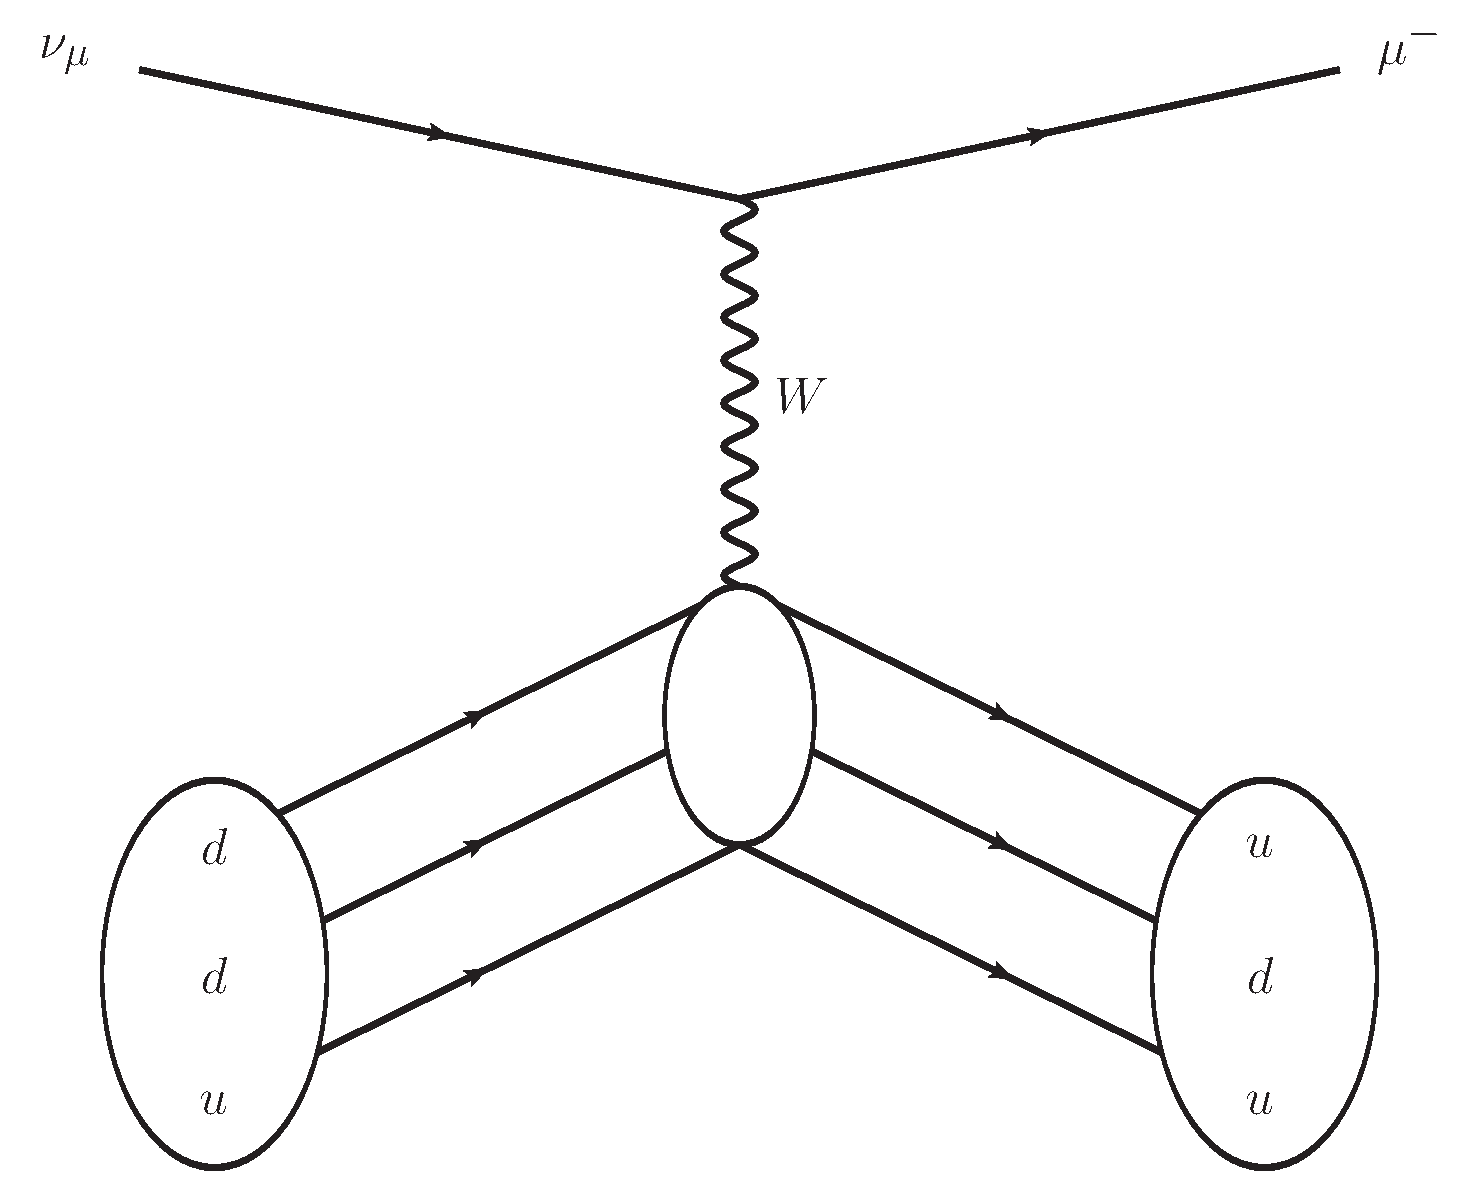
\includegraphics[width=8cm]{images/neutrino_interactions/CCQE_FD.eps} \label{fig:CCQEFD}}
  \subfloat[NCQE.]{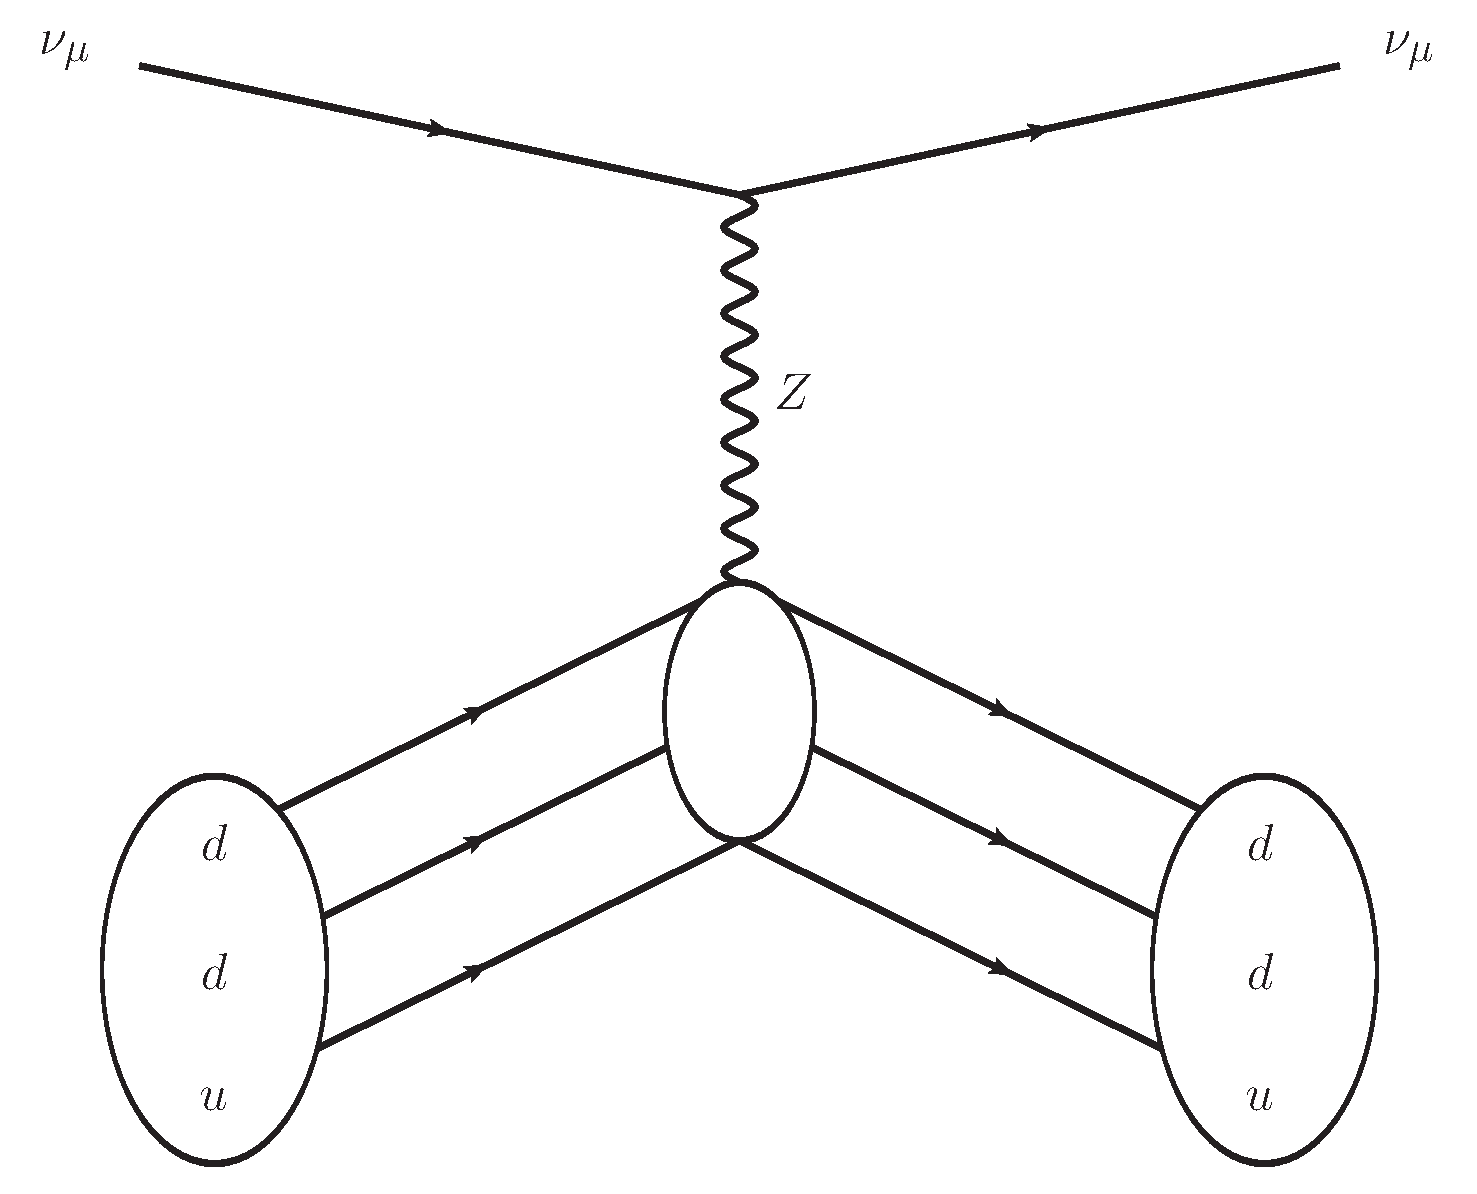
\includegraphics[width=8cm]{images/neutrino_interactions/NCQE_FD.eps} \label{fig:NCQEFD}}
  \caption{Quasi-Elastic (QE) interactions of a $\nu_\mu$ with a nucleon.  The small ellipse represents the neutrino interacting with the nucleon as a whole, rather than with an individual parton.}
  \label{fig:QEFD}
\end{figure}
\newline
\newline
For higher energy neutrinos, there is sufficient energy to promote the target nucleon to an excited state.  A quick after-effect of this promotion is that the excited state decays, resulting in further particle emission.  This interaction topology, which dominates in the 1~GeV to 5~GeV energy range, is known as RESonant pion (RES) production as the neutrino interaction produces $\Delta$ resonance which typically decays to a nucleon and a single pion in the final state.  In the case of $\nu_\mu$ CCRES, the interaction generally takes the following form
\begin{equation}
\nu_\mu N \rightarrow \mu^- N^{*},
\label{eq:CCRES}
\end{equation}
\begin{equation}
N^{*} \rightarrow \pi N',
\end{equation}
where $N, N' = n, p$.  An example diagram of a $\nu_\mu$-CCRES interaction with a $\pi^+$ in the final state is shown in Fig.~\ref{fig:CCRESFD}.
\begin{figure}%
  \centering
  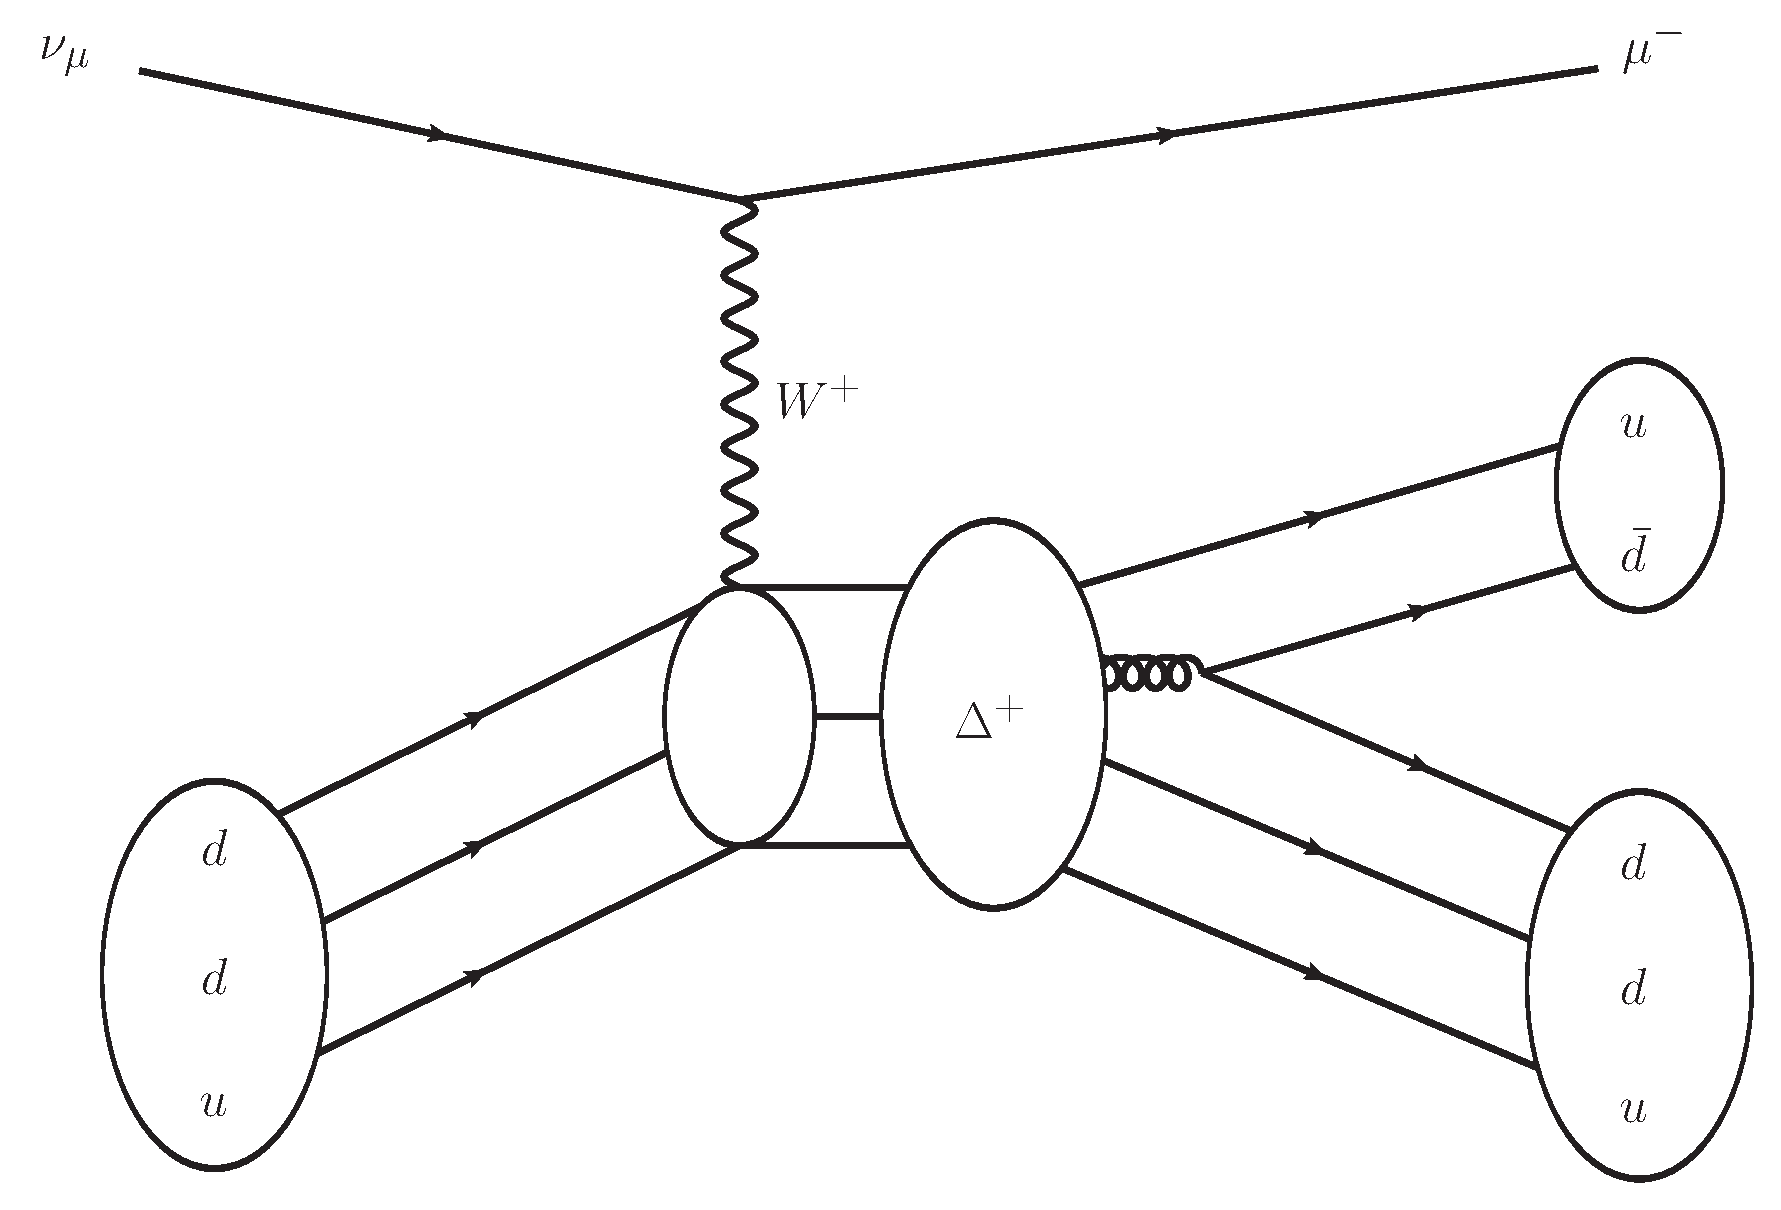
\includegraphics[width=8cm]{images/neutrino_interactions/CCRES_FD.eps}
  \caption{A Charged Current RESonant pion (CCRES) interaction of a $\nu_\mu$ with a neutron.  The $\Delta$ resonance decays to a neutron and a $\pi^+$.}
  \label{fig:CCRESFD}
\end{figure}
\newline
\newline
For neutrinos with energy above the RES-dominant region, the neutrino has enough energy to penetrate the nucleon and scatter off an individual quark.  Because of the nature of the strong force, the scattered quark and the nucleon remnant produce a hadronic shower in the final state.  This process is known as Deep Inelastic Scattering (DIS).  For $\nu_\mu$-CCDIS, the interaction takes the following form
\begin{equation}
\nu_\mu N \rightarrow \mu^- X,
\label{eq:CCDIS}
\end{equation}
where $X$ is the remnant of the nucleus after the interaction occurs.  An example diagram of a $\nu_\mu$-CCDIS interaction is shown in Fig.~\ref{fig:CCDISFG}.
\begin{figure}%
  \centering
  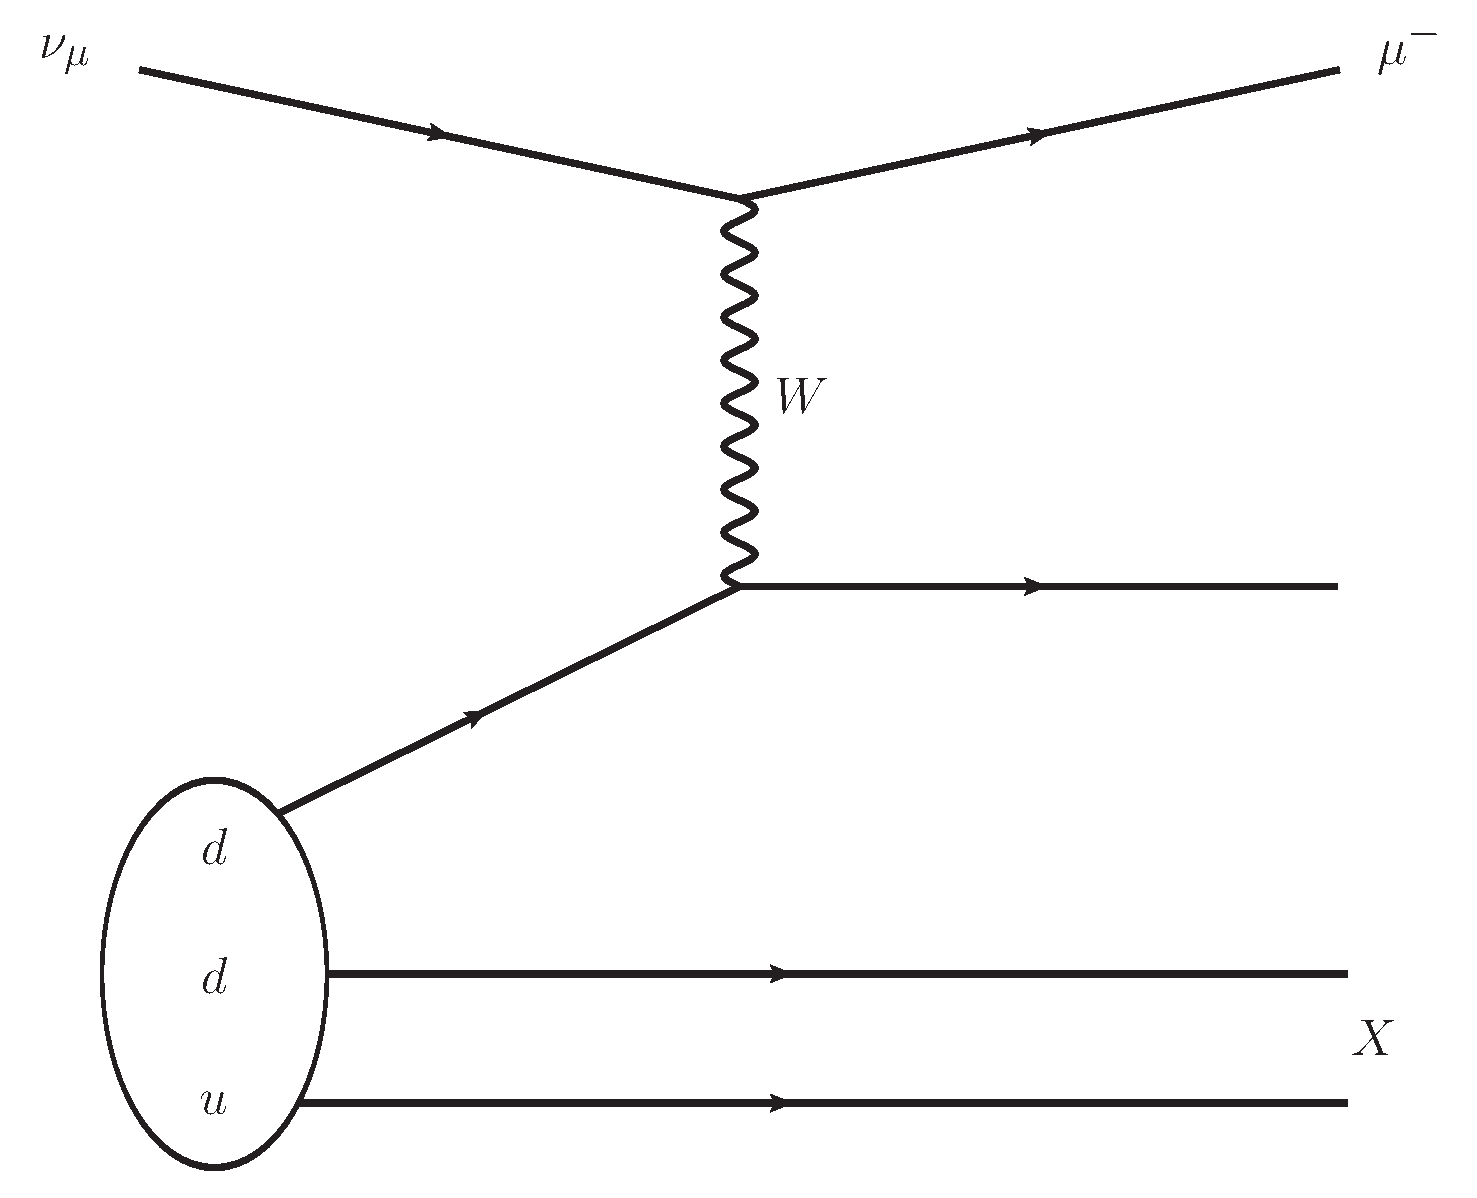
\includegraphics[width=8cm]{images/neutrino_interactions/CCDIS_FD.eps}
  \caption{A Charged Current Deep Inelastic Scattering (CCDIS) interaction of a $\nu_\mu$ with a neutron. $X$ \Yoshi{represents}{ADDRESSED - was `resembles'} the leftover nuclear remnant.}
  \label{fig:CCDISFG}
\end{figure}
\newline
\newline
While the value of a particular interaction cross-section should depend on the nuclear environment, it is possible to make comparisons of the measured cross-section per nucleon.  Fig.~\ref{fig:CrossSectionMeasurements}\Yoshi{}{Make this figure bigger. Say something about the data points as well as the curves, and how up-to-date it is etc.} shows a comparison of $\nu_\mu$ CC cross-section measurements per nucleon from different experiments, all of which sample a different neutrino energy range.  There are large uncertainties for many of the cross-section measurements, particularly for the ones sampling the lower energy ranges.  The T2K beam energy is $\sim$700~MeV, which sits in the region of higher uncertainty.
\begin{figure}[b]%
  \centering
  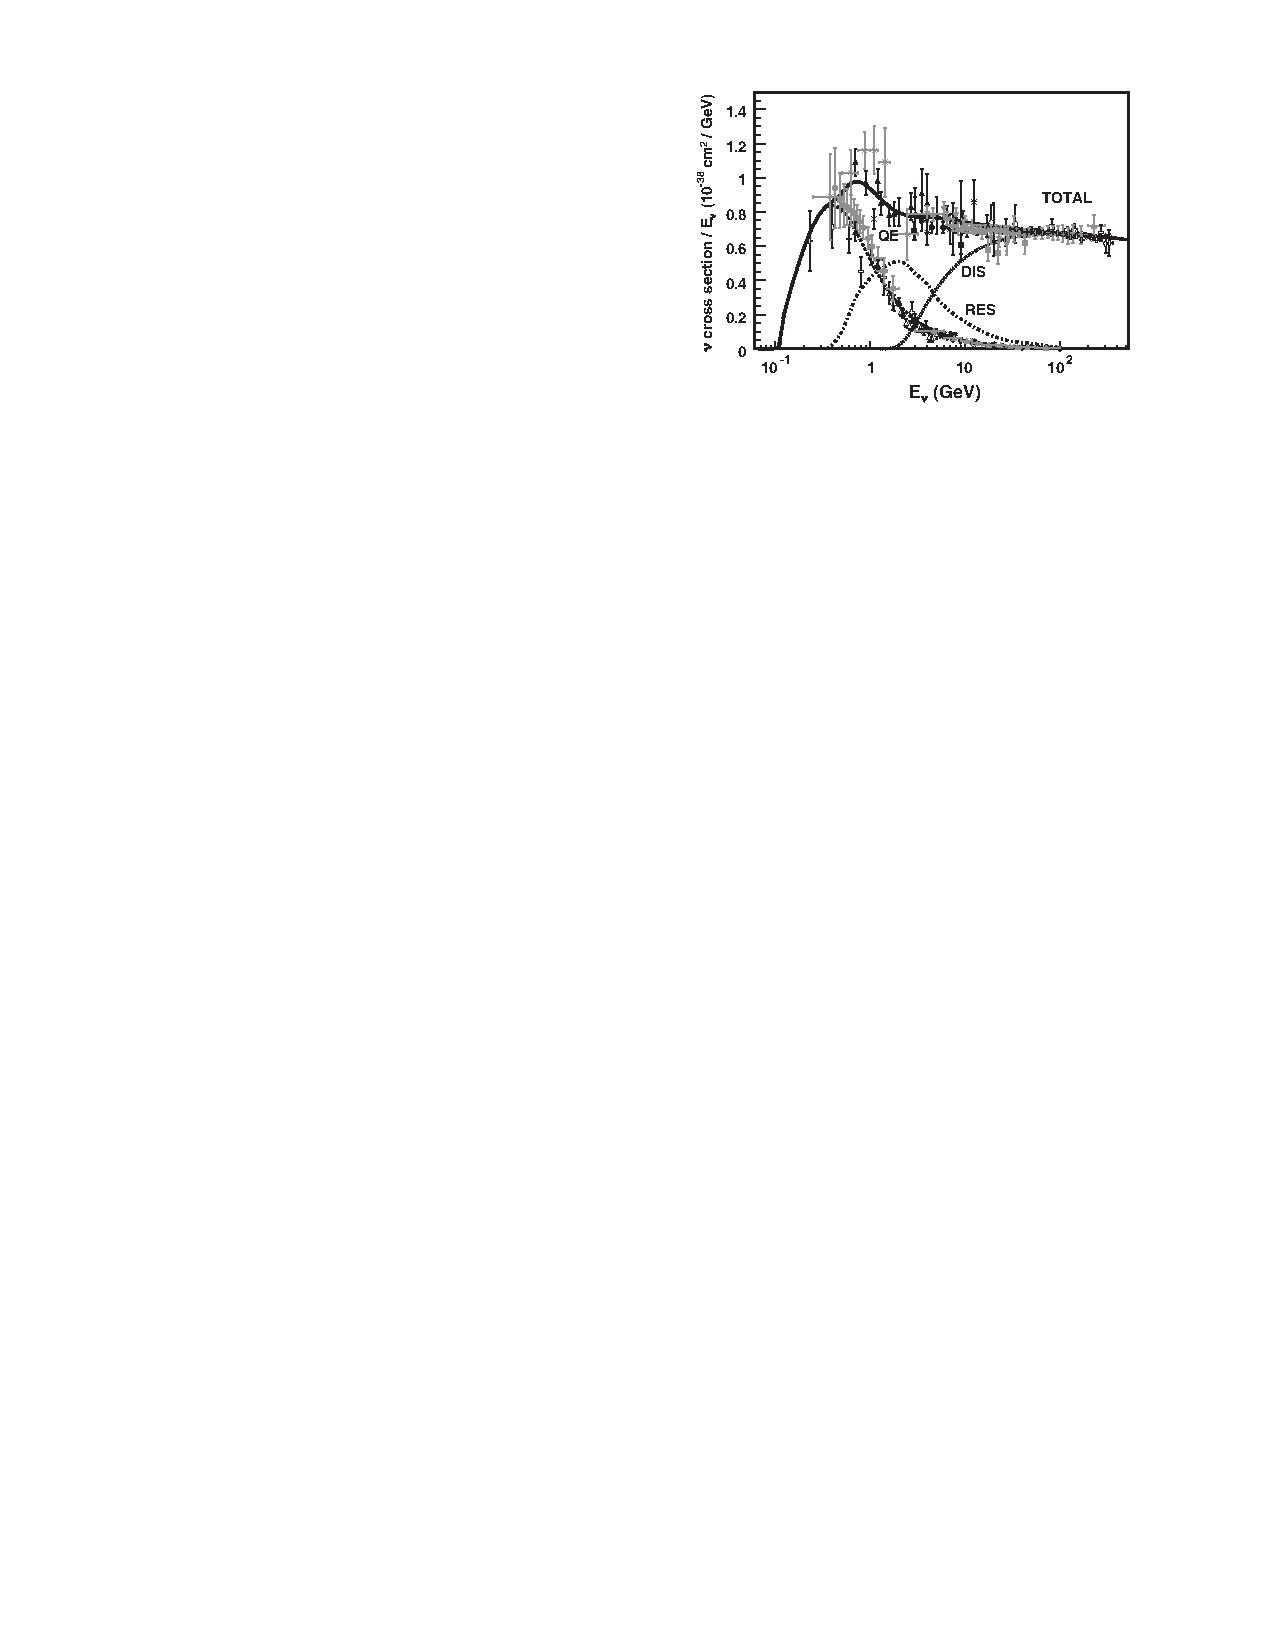
\includegraphics[width=12cm]{images/neutrino_interactions/CrossSectionMeasurements.pdf}
  \caption{$\nu_\mu$ CC cross-section measurements per nucleon and divided by neutrino energy for a range of energies, showing the QE, RES and DIS contributions~\cite{RevModPhys.84.1307}.  The data points are provided by a range of experiments (from 1979 to 2010) including BEBC~(1979)~\cite{Colley:1979rt}, NuTeV~(2006)~\cite{PhysRevD.74.012008}, MINOS~(2010)~\cite{PhysRevD.81.072002} and others.  The example predictions are provided by the NUANCE generator~\cite{Casper:2002sd}.  Many measurements have a large associated uncertainty, particularly in the lower energy (less than 1~GeV) regime.  The heaviest target nucleus probed in the region of interest, near 1~GeV, is carbon.}
  \label{fig:CrossSectionMeasurements}
\end{figure}
\newline
\newline
CCQE interactions are experimentally the most interesting and this is the interaction region where most recent measurements have been focused.  Because of the simplicity of the CCQE topology, the interaction can be treated as a two-body scatter.  So, by applying simple conservation rules, the neutrino energy can be kinematically reconstructed.  In such interactions, the nucleon structure is parameterised using a set of form factors, the most interesting of which is the axial-vector form factor, $F_A(Q^2)$. $F_A(Q^2)$ has been, and still is, assumed to take a dipole form
\begin{equation}
F_A(Q^2) = \frac{F_A(0)}{(1-Q^2/M_A^2)^2}
\label{eq:FAFormFactor},
\end{equation}
where $Q^2$ is the negative of the squared four-momentum transfer of the lepton to the hadron, $F_A(0) = 1.2694\pm0.0028$~\cite{0954-3899-37-7A-075021}, and $M_A$ is known as the axial mass.  Recent measurements of the CCQE cross-section by the MiniBooNE~\cite{PhysRevD.81.092005} and NOMAD~\cite{NOMAD-CCQE} experiments have sparked interest by reporting measured cross-sections which are in tension with one another, the results of which shown in Fig.~\ref{fig:CCQECrossSectionMiniBooNENOMAD}.  
\begin{figure}%
  \centering
  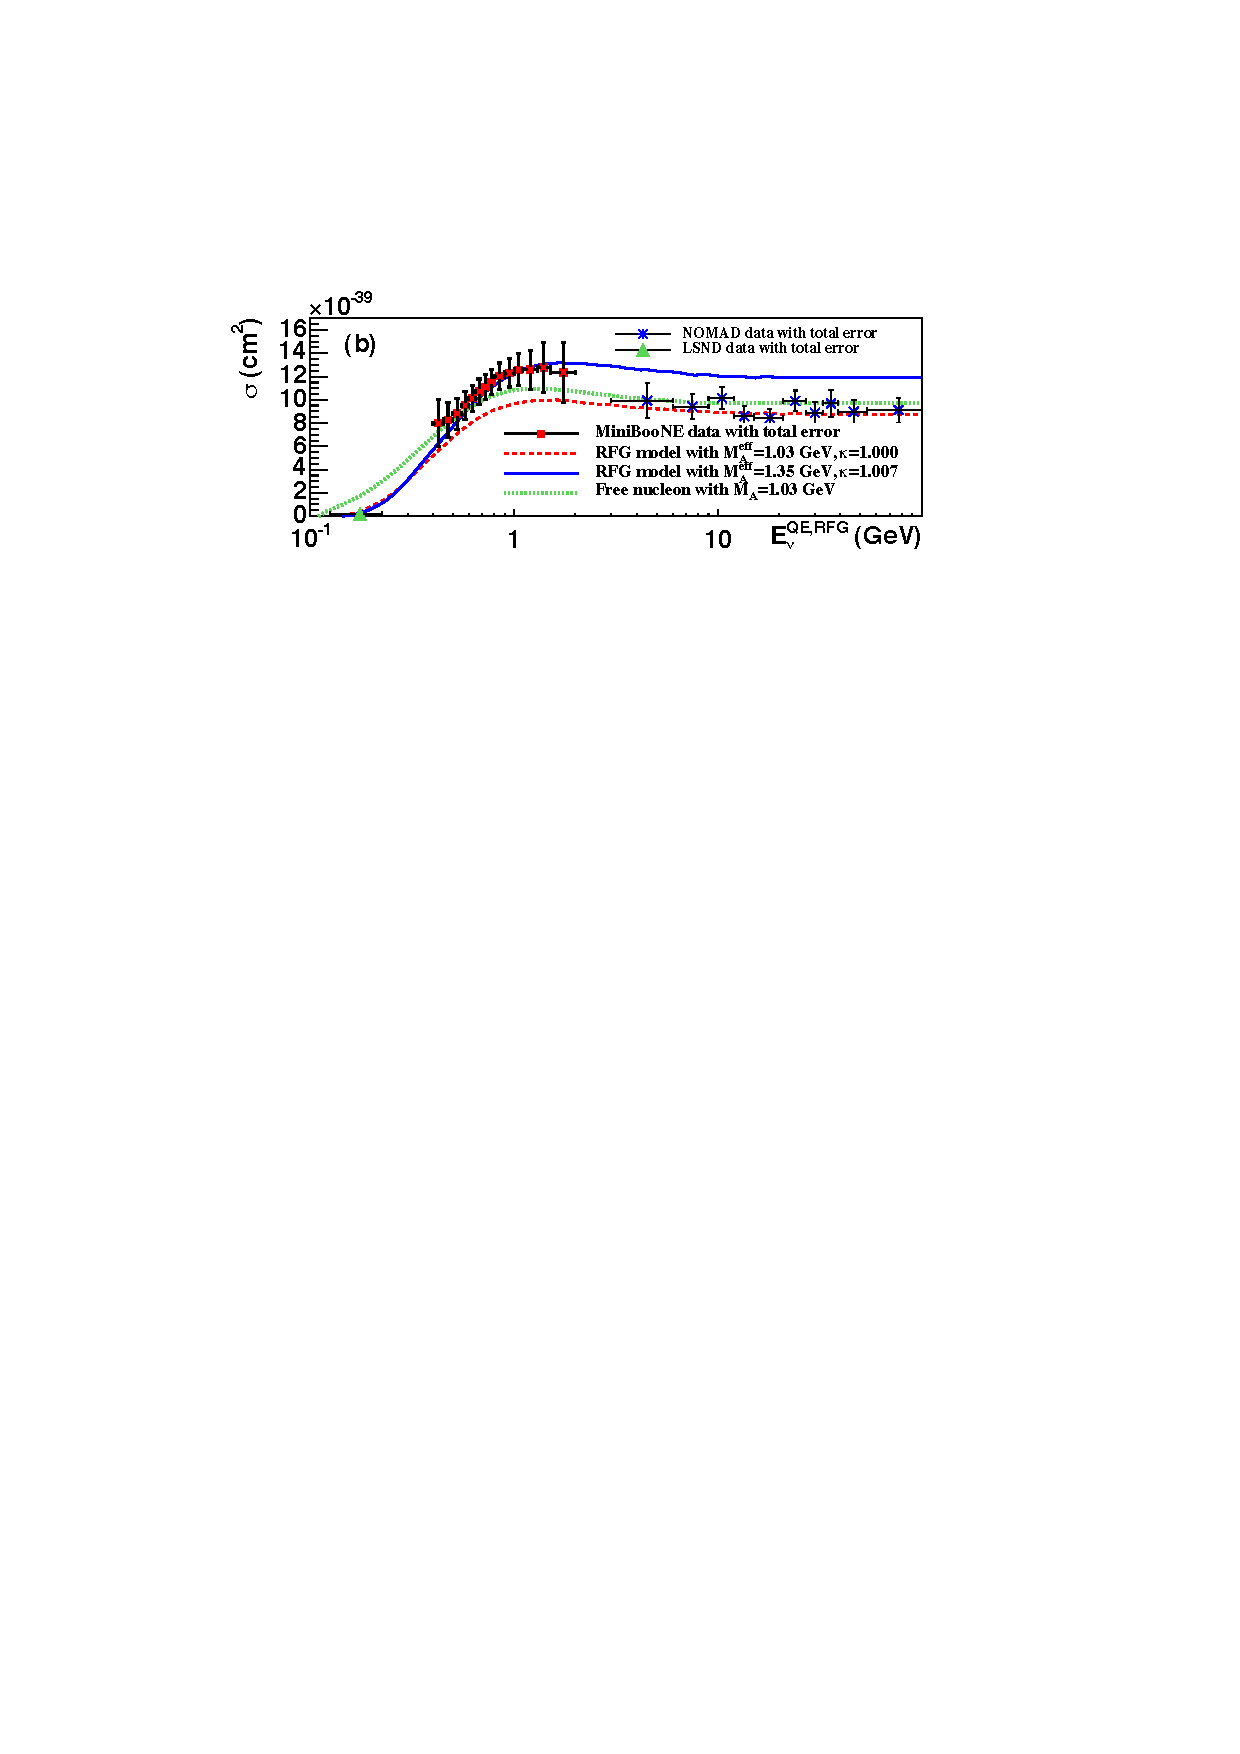
\includegraphics[width=12cm]{images/neutrino_interactions/CCQECrossSectionMiniBooNENOMAD.pdf}
  \caption{The CCQE cross-sections measured by the MiniBooNE~(2010)~\cite{PhysRevD.81.092005}, LSND~(2002)~\cite{Auerbach:2002iy} and NOMAD~(2009)~\cite{Lyubushkin:2008pe} experiments.  The solid and dashed lines represent predictions from the NUANCE generator with different values of $M_A$~\cite{PhysRevD.81.092005}.  Each prediction does not well model all of the data shown in the figure, indicating tension between the data collected by each of the experiments.}
  \label{fig:CCQECrossSectionMiniBooNENOMAD}
\end{figure}
A popular explanation for this discrepancy is a lack of understanding of the nuclear environment.  Because the neutrino is not scattering of a free nucleon, but rather a nucleon in a strongly contained system, experiments actually measure an effective $M_A$.  It is possible that the nuclear effects cause a modification to the effective $M_A$ that the experiments measure.  This possible explanation for the discrepancy has placed a heavier emphasis on nuclear modelling in neutrino interaction experiments. 
\section{Neutrino interactions with heavy nuclei}
\label{sec:NeutrinoInteractionsHeavyNuclei}
As introduced above, consideration of nuclear effects in cross-section measurements is important.  This is especially true for neutrino interactions on heavy target nuclei.  As one can imagine, the presence of a nucleus can dramatically effect the interactions that are observed in a detector.  A popular model for the nucleus is the Relativistic Fermi-Gas (RFG) model~\cite{Smith:1972xh}.  The RFG model treats the nucleus as a collection of non-interacting nucleons sitting in a potential well.  The nucleons are stacked in the potential well according to the Pauli exclusion principle.  This leads to a uniform momentum distribution of the nucleons up to the Fermi momentum $p_F$.  Importantly, the Pauli exclusion principle has a further effect.  Because the final state nucleon is forbidden from occupying a state taken by another nucleon in the potential well, the energy transfer of the neutrino to the nucleon must result in a final state nucleon with a momentum above $p_F$, resulting in a reduction of the cross-section.
\newline
\newline
The RFG can only model the effect of the nucleus on the initial neutrino interaction which creates the final states.  However, these final states are created within the nucleus and so additional interactions of the final states with the nucleus can occur.  The Final-State Interactions (FSI) can significantly alter the momentum and direction of the final-state particles.  As the final-state particles are used to infer neutrino properties, the FSI effects can alter the interpretation of the reconstructed events.  In simulation, variations of the cascade model are typically used.  This involves pushing the final-state particles through the nucleus in discreet steps and, at each step, probabilistically updating the particle properties.  If at any point a final-state particles knocks out another nucleon, the additional nucleon is also pushed through the nucleus in parallel.  The discreet stepping occurs until all relevant particles have escaped the nucleus.
\newline
\newline
To test such cross-section models, including nuclear effects, it is necessary to compare prediction with collected data.  However, collected cross-section data for heavy nuclei is relatively sparse.  In the case of lead, only two experiments have performed cross-section measurements.  The first measurement was performed by the CHORUS~\cite{CHORUS_XSEC} experiment in 2003.  The CHORUS detector, exposed to the CERN SPS beam with a wide-band $\nu_\mu$ beam of 27~GeV average energy, measured a cross-section for lead, iron, marble and polyethylene.  However, because the absolute flux was not measured in the experiment, all of the cross-section measurements were normalised to a common constant.  Their results are summarised in Fig.~\ref{fig:CHORUSXSec}\Yoshi{}{ADDRESSED - ``data/prediction'' is confusing because it looks like the ratio of the two. Say which experiment is, and when the data was taken, in the caption, not just the body text}.
\begin{figure}%
  \centering
  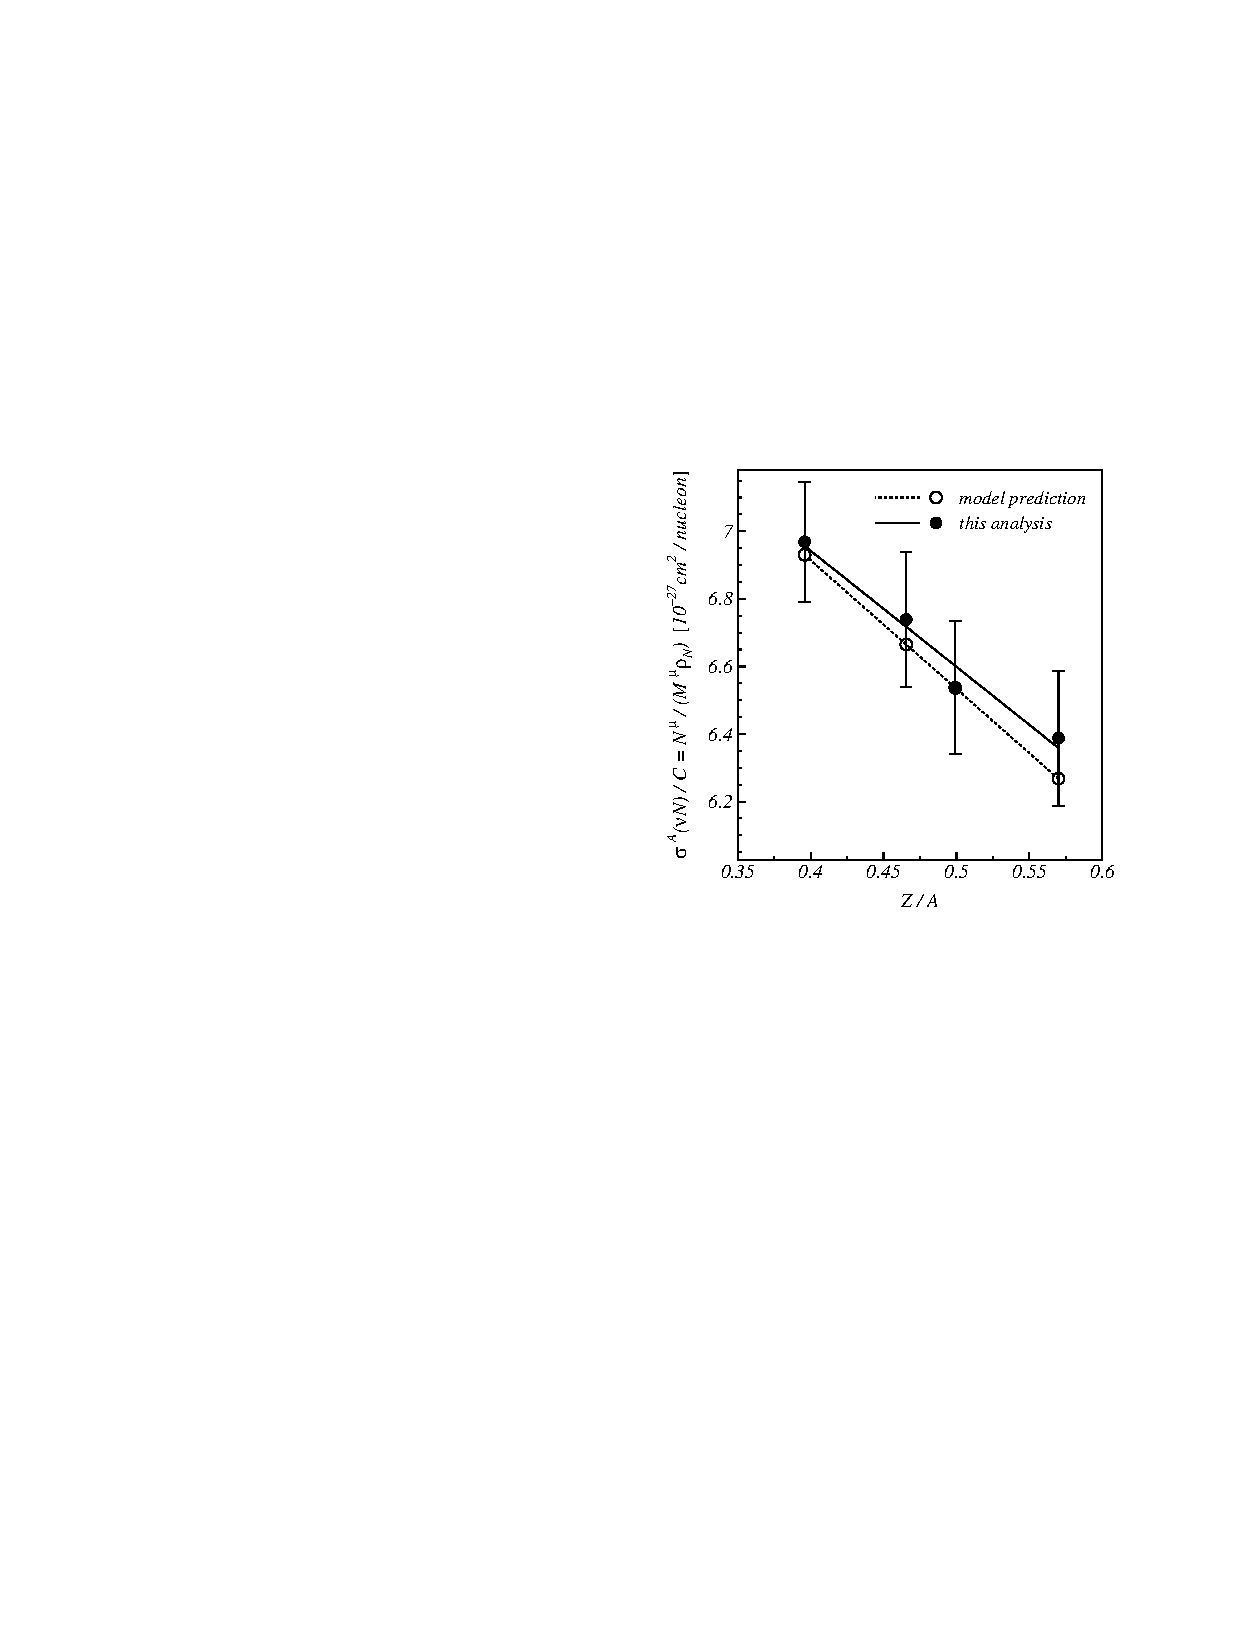
\includegraphics[width=8cm]{images/neutrino_interactions/CHORUS_XSec.pdf}
  \caption{Measured values of the $\nu_\mu$ CC relative cross-section for several elements, as measured by the CHORUS experiment~(2003)~\cite{CHORUS_XSEC}.  The black and white points are the collected data and prediction respectively.  The solid and dashed lines are the linear best fit lines to the data and prediction respectively.  Going from left to right, the points represent data and prediction for lead, iron marble and polyethylene.  The prediction is taken from a set of quark distribution functions~\cite{Gluck:1998xa} provided by PDFLIB.}
  \label{fig:CHORUSXSec}
\end{figure}
The second measurement was made by the MINER$\nu$A experiment~(2014)~\cite{PhysRevLett.112.231801}, which used the Fermilab NuMI beam with a 8~GeV average energy, to measure the relative $\nu_\mu$ CC cross-section on lead to that of plastic scintillator as a function of neutrino energy.  Their results, shown in Fig.~\ref{fig:MINERvAXSec}, largely agreed with the prediction.  The energy sampled is above the 1~GeV region of interest.
\begin{figure}%
  \centering
  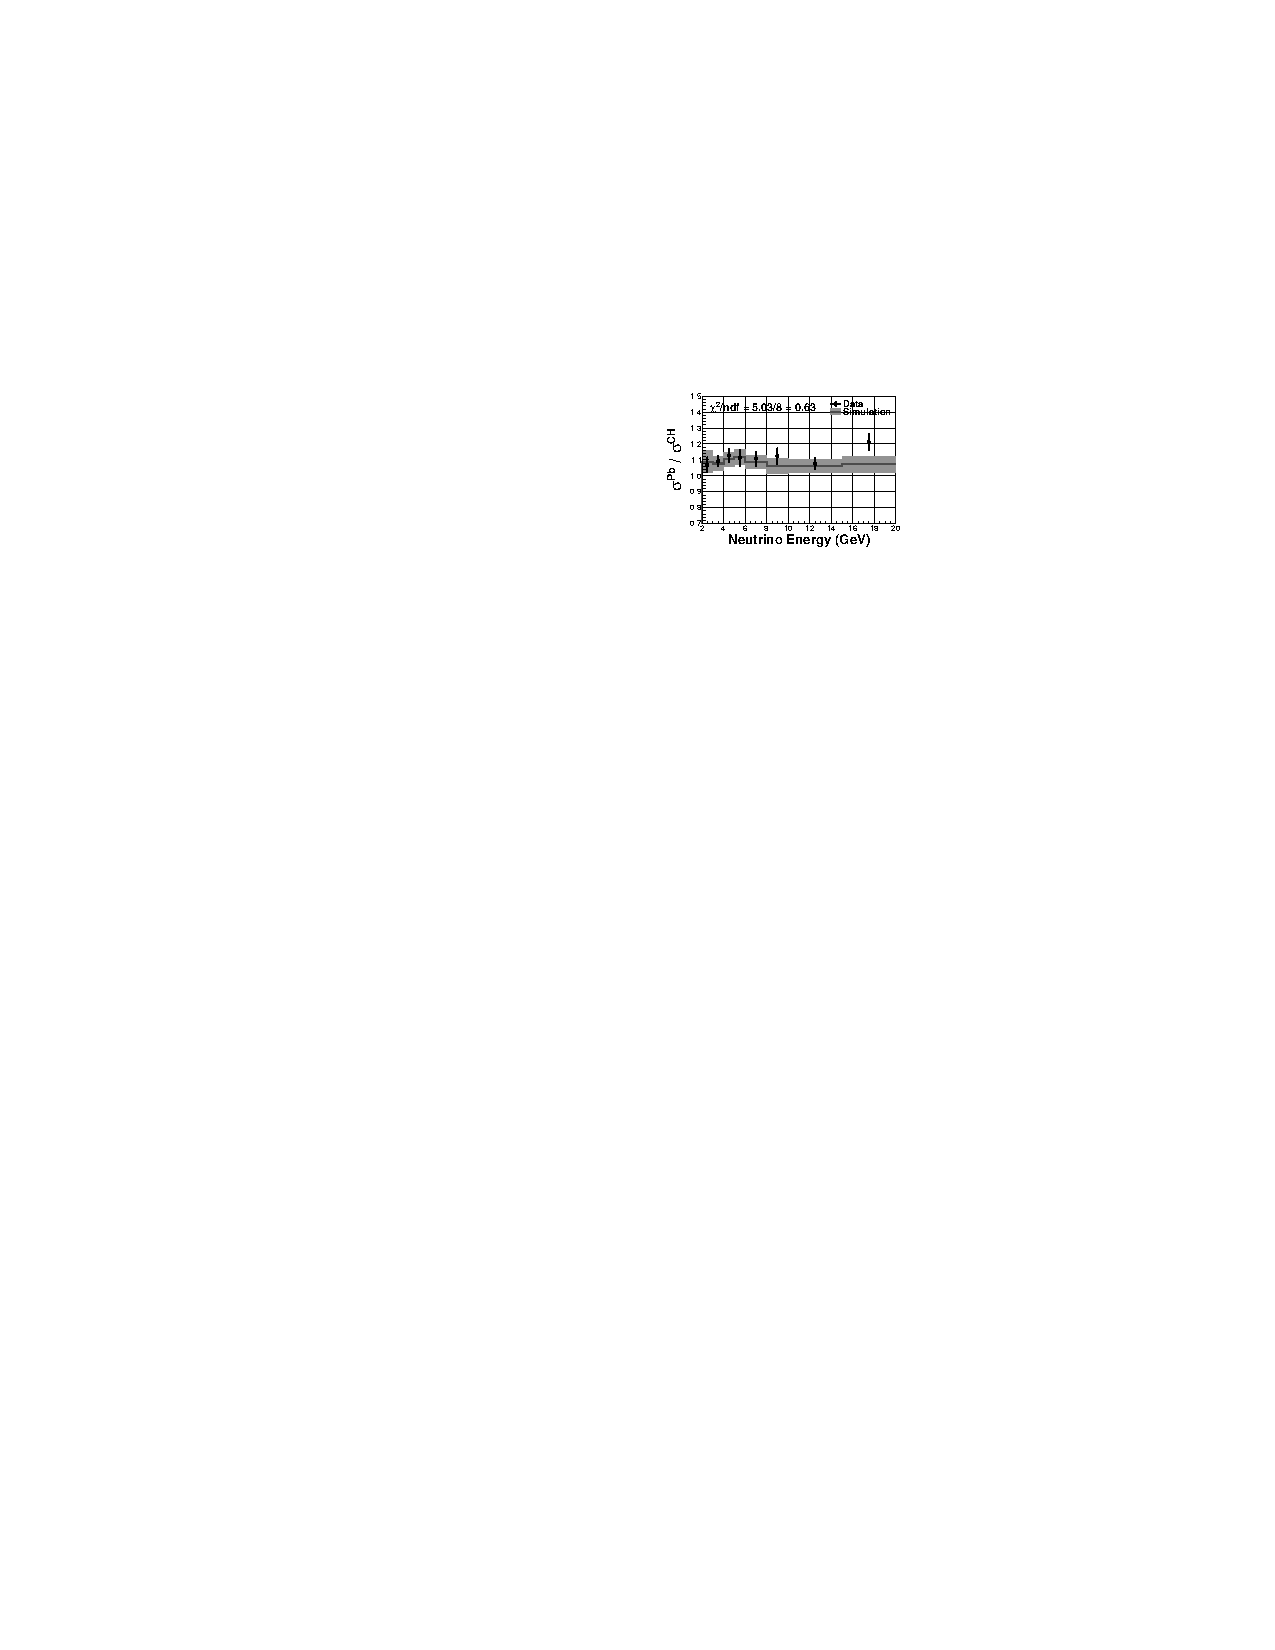
\includegraphics[width=10cm]{images/neutrino_interactions/MINERvA_XSec.pdf}
  \caption{Ratio of the measured $\nu_\mu$ CC inclusive cross-section on lead to plastic scintillator as a function of neutrino energy, as measured by the MINER$\nu$A experiment~(2014)~\cite{PhysRevLett.112.231801}.  The simulation is based on the GENIE generator~\cite{Andreopoulos201087}.  The error bars on the simulation (data) are statistical (systematic) uncertainties.\Yoshi{}{ADDRESSED - WHAT EXPERIMENT IS THIS? Your captions are generally lacking---they need to stand on their own, without the need for the reader to find the corresponding body text to figure out what a plot is about.}}
  \label{fig:MINERvAXSec}
\end{figure}
\newline
\newline
As neutrino oscillation physics has entered the precision era\Yoshi{}{ADDRESSED - We entered the precision era quite a while ago---see KamLAND's mixing angle error!}, it has become very important that our understanding of neutrino cross-sections improves.  To achieve this goal, more cross-section measurements across a range of nuclear targets are needed.  This thesis presents a measurement of the $\nu_\mu$ CC inclusive cross-section on lead using the electromagnetic calorimeters contained in the near detector of the T2K experiment.  

